
\chapter{网内业务分析}
\section{排队论基础}
\textbf{资源的有限性} 和\textbf{ 需求的随机性} 是 排队现象存在的基础;\\
由于 顾客到达 和 服务完毕的时间 都是 不确
定 的,绝大多数排队系统工作于 随机状态。
\subsection{排队论的概念}
\subsubsection{基本概念}
\subsubsubsection{三个参数}
\begin{itemize}
 	\item  服务员数目m
 	\item 顾客到达率 $\lambda$,单位时间内平均到达排队系统的顾客数量
 	 ,相邻两顾客到达的时间间隔$t$,其$\textnormal{统计平均值}\overline{t}=\frac{1}{\lambda}$
 	\item 服务员服务速率$\mu$ ,顾客服务时间$\tau$,其统计平均值为$\overline{\tau}=\frac{1}{\mu}$\begin{itemize}
 		\item m = 1,$\mu$为服务速率
 		\item m >1 ,$m\mu$为服务速率
 	\end{itemize}
\end{itemize}
	\subsubsection{一般性质}
	\begin{itemize}
		\item 平稳性,在时间间隔t内,到达 到达k 个顾客的概率只与t的长 的长
		度 有关,而与这间隔的起始时刻无关。
		\item 无后效性,顾客到达时刻互相独立,即顾客各自独立地
		随机到达。
		\item 疏稀性,在$\delta t$ 内只有一个顾客到达或没有顾客到达。
	\end{itemize}
	满足上三个条件的随机流成为\textbf{简单流},简单流的到达间隔是负指数分布,在一段时间内到达的顾客数服从泊松分布。
	\subsubsection{到达时间分布}
\begin{figure}[H]
	\centering
	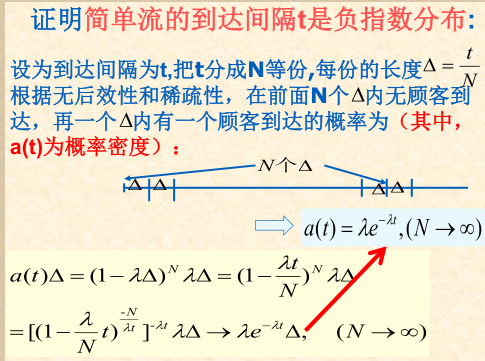
\includegraphics[width=0.5\linewidth]{figures/prove_1}
	\caption{}
	\label{fig:prove1}
\end{figure}
\begin{figure}[H]
	\centering
	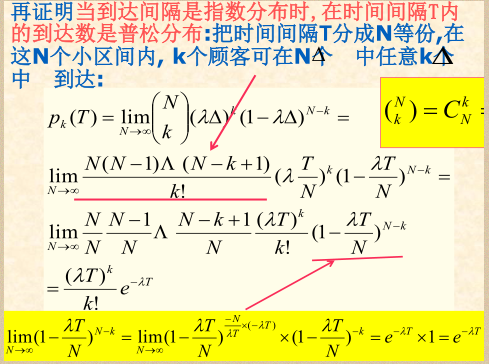
\includegraphics[width=0.5\linewidth]{figures/prove_2}
	\caption{}
	\label{fig:prove2}
\end{figure}
(0,t)时间内有顾客达到的概率:$p = 1- p_0(t) = 1 - e^{-\lambda t}$,即1-(0,t) 时间内没有人到达的概率\\
所以,对于简单流:
\begin{gather}
	\text{概率密度:}a_T(t) = \begin{cases}
	\lambda e^{-\lambda t}, t>0 \\
	0,t\le 0
	\end{cases} \\
	\text{分布函数:}F_T(t) = \begin{cases}
	1 - e^{\lambda t},t>0 \\
	0,t\le 0
	\end{cases}
\end{gather}
这里分布函数表示\textbf{t}时间内有顾客到达的概率.
\subsubsection{服务时间分布}
同到达时间,只用将字母$\lambda \textnormal{换成} \mu$
\subsubsection{排队系统表示方式}
$A | B | m(N,n) $
\begin{itemize}
	\item A--顾客到达时间间隔分布
	\item B--服务时间间隔分布
	\item m--窗口数
	\item N--潜在顾客数
	\item n--截止队长
\end{itemize}
\subsubsection{常见几种分布}
\begin{enumerate}
	\item M分布
	\item $E_r$分布,适用于成批处理的排队。
	\item $D$分布,冲激
	\item $E_r,D$分布
	\item $H_R$分布,R阶指数分布
\end{enumerate}
\subsection{系统的工作方式}
排队系统的运行性能不仅与上述的统计分布
有关,还与系统预先规定的 工作方式有关 。
\begin{itemize}
	\item 排队规则 是指服务机构是否允许排队
	\item  服务规则 是指在排队等待情形下 服务的顺
	序 是什么
\end{itemize}
\subsubsection{排队规则}
\begin{figure}[H]
	\centering
	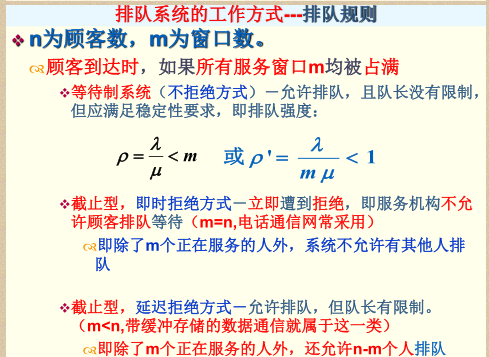
\includegraphics[width=0.7\linewidth]{figures/prove_3}
	\caption{}
	\label{fig:prove3}
\end{figure}
\subsubsection{服务规则}
\begin{itemize}
	\item 先到先服务
	\item 后到先服务
	\item 优先制服务
	\item 随机服务
\end{itemize}
\subsection{主要性能指标}
%\begin{figure}[H]
%	\centering
%	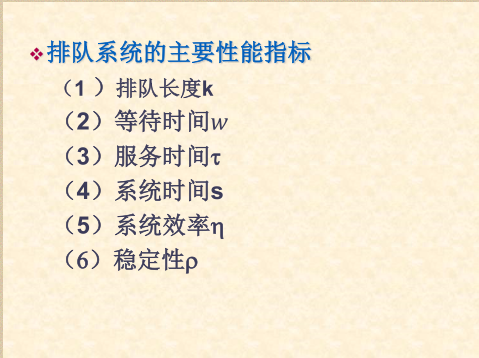
\includegraphics[width=0.5\linewidth]{figures/prove_4}
%	\caption{}
%	\label{fig:prove4}
%\end{figure}
\begin{description}
	\item[排队队长K] 系统中\textbf{滞留的顾客数},包括\textbf{正在服务的顾客}。\\
	三种观察模式:
	\begin{enumerate}
		\item $ p_k $随机观察
		\item $ r_k $顾客到达时观察
		\item $ d_k $顾客离开时观察
	\end{enumerate}
	\begin{itemize}
		\item 当顾客的到达规律服从马尔科夫性,$ p_k = r_k $
		\item 每个瞬间只能离开一个人时,则$ r_k = d_k $
		\item 满足稀疏性,只要顾客达到是泊松流。$ p_k = r_k = d_k $
	\end{itemize}
	\item[等待时间$ w $] 顾客到达至开始被服务这段时间,在通信网中,等待时延是\textbf{平均时延的主要组成部分},其它时延一般为常亮,而且比较小。
	\item[服务时间$ \tau $] 
	\item[系统时间$ s $] 系统从到达至离开这段时间。$ s = w+\tau$\\
	\textbf{Little 公式}
	\begin{equation}\label{key}
	k = \lambda s
	\end{equation}
	\item[系统效率$ \eta $] 定义为平均窗口占有率。某时刻t有$ r_t $个窗口被占用,共有m个窗口,则\begin{equation}\label{key}
	\eta_t = \frac{r_t}{m}
	\end{equation}
	$ \eta_t $的统计平均值就是系统效率。
	\begin{equation}\label{key}
	\eta = \frac{r}{m}
	\end{equation}
	\begin{equation}\label{key}
	\eta = \begin{cases}
	\rho,\text{单窗口}\\
	\frac{\overline{r}}{m},\text{多窗口}
	\end{cases}
	\end{equation}
	\item[稳定性] 	\hspace{1pt}
	\begin{itemize}
		\item 不拒绝系统,$ \rho = \frac{\lambda}{m\mu} $小于1稳定,大于等于1不稳定
		\item 拒绝系统,稳定。
	\end{itemize}
\end{description}
\subsection{M|M|1问题求解}
求解步骤:
\begin{enumerate}
	\item 确定状态变量,常用的是队长k
	\item 画出状态转移图
	\item 列出状态转移方程
	\item 求解状态转移方程
\end{enumerate}
\subsubsubsection{差微分方程}
\begin{itemize}
	\item 写出$ t $到$ (t+\Delta t) $之间的顾客数为k转移情况
	\item 忽略高次
	\item 求解微分
	\begin{figure}
		\centering
		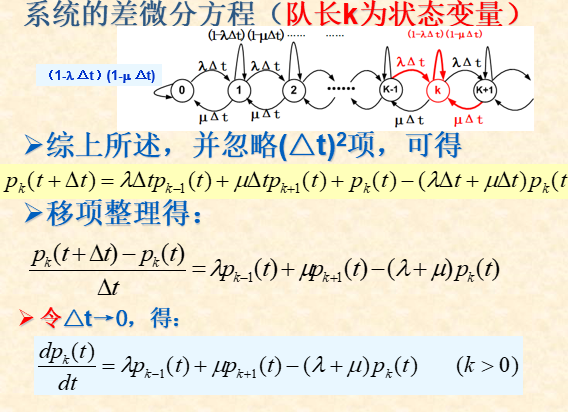
\includegraphics[width=0.7\linewidth]{figures/screenshot025}
		\caption{}
		\label{fig:screenshot025}
	\end{figure}
\end{itemize}
\textbf{注意:方程列些的除了一般情况,还要考虑特殊状态:如k为0,k等于服务台个数m,k等于截止队长个数等}\\
哥尔摩克罗夫方程:
\begin{equation}\label{key}
dp_k(t)=(dt\text{内进入k状态的概率})-(dt\text{内离开k状态的概率})
\end{equation}
分析排队系统,就是解这些系统方程。有\textbf{稳态解和暂态解},当t->$ \infty $,$ p_k(t) $已经稳定。此时$ \frac{dp_k(t)}{dt} =0$,记为$ p_k $
\subsubsubsection{稳态方程}
\begin{figure}
	\centering
	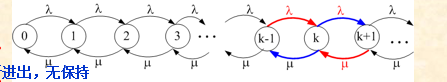
\includegraphics[width=0.7\linewidth]{figures/screenshot027}
	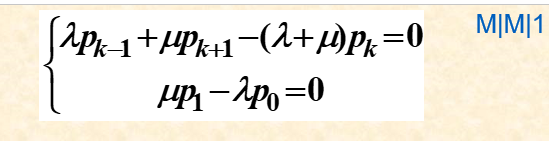
\includegraphics[width=0.7\linewidth]{figures/screenshot028}
	\caption{}
	\label{fig:screenshot027}
\end{figure}
\begin{equation}\label{key}
\text{出} = \text{入}
\end{equation}
\subsubsection{M|M|1 参数求解}
需要注意的是,所有公式都建立在$ \rho \le 1 $的情况下,因为M|M|1是不拒绝系统,$ \rho \ge 1 $不能使系统稳定工作。
\begin{figure}[H]
	\centering
	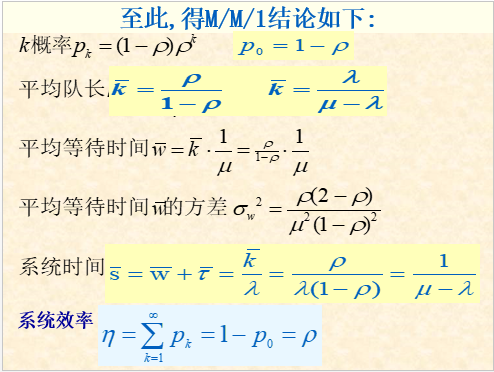
\includegraphics[width=0.5\linewidth]{figures/prove_5}
	\caption{}
	\label{fig:prove5}
\end{figure}
\subsubsection{M|M|1 闲期和忙期}
\begin{figure}[H]
	\centering
	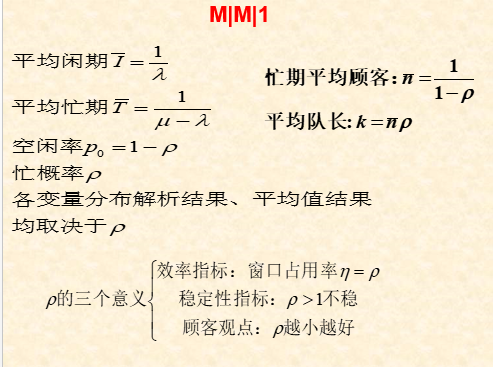
\includegraphics[width=0.5\linewidth]{figures/prove_6}
	\caption{}
	\label{fig:prove6}
\end{figure}
\subsubsection{通信网中的排队论计算}
\textbf{计算通信网中的M/M/1系统指标,将原来的$\mu$ 换为$\mu C$}
\begin{enumerate}
	\item $ \frac{1}{\mu} $为分组长度,单位为bit
	\item $ C $信道容量,单位为bit/s
	\item 则发送时间间隔为$ \frac{1}{\mu C} $,即发送速率为$ \mu C $,如果有m条信道,则发送速率为$ m\mu C $
\end{enumerate}
\begin{figure}[H]
	\centering
	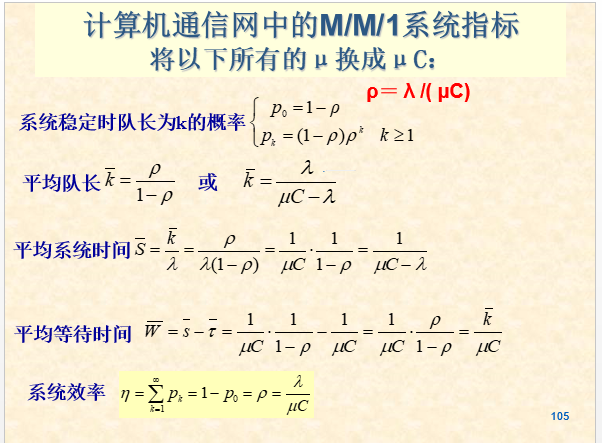
\includegraphics[width=0.7\linewidth]{figures/screenshot026}
	\caption{}
	\label{fig:screenshot026}
\end{figure}
\subsection{M|M|m(n)}
压缩排队长度的措施:
\begin{itemize}
	\item 增加窗口数
	\item 截止排队长度
\end{itemize}

融合上述两种方式,成为\textbf{截止型多窗口排队系统}\\
\begin{itemize}
	\item 混合排队方式,顾客排成一个队,接受m个窗口的服务
	\item 分别排成m个队
\end{itemize}
状态转移图及稳态方程:
\begin{figure}[H]
	\centering
	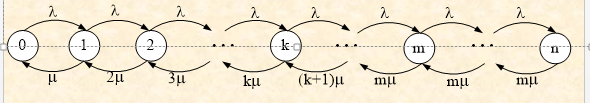
\includegraphics[width=0.7\linewidth]{figures/screenshot029}
	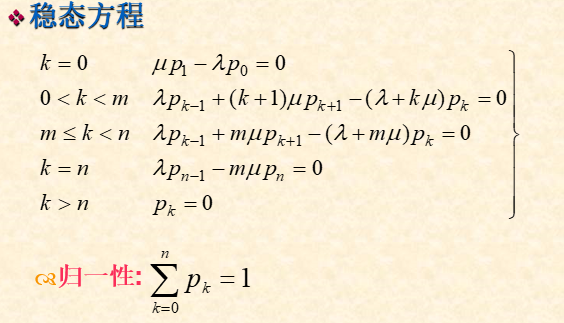
\includegraphics[width=0.7\linewidth]{figures/screenshot030}
	\caption{}
	\label{fig:screenshot029}
\end{figure}
\textbf{不要忘记k>n的情况。}


\textbf{即时拒绝系统的拒绝概率(爱尔兰公式)}
\[
 	p_n = \frac{a^m/{m!}}{\sum_{r=0}^{m}a^r/{r!}}
\]
\begin{itemize}
	\item a为呼叫量(话务量)
	\item m,线路条数
\end{itemize}
\subsubsection{业务量和呼叫量}
\textbf{业务量}是在\textbf{指定时间内线路被占用的总时间},其量纲为时间\\
基于排队论的\textbf{话务量}:
\begin{equation}\label{key}
Y = \lambda S T
\end{equation}
\begin{itemize}
	\item $ \lambda $单位时间发生呼叫的次数
	\item S:每次呼叫占用的时间
	\item T:考察时间
\end{itemize}
\textbf{呼叫量}定义为\textbf{线路占用时间和观察时间之比},即业务量的强度。
\begin{equation}\label{key}
\text{呼叫量} = \frac{\text{业务量}}{\text{观察时间}}
\end{equation}
单位为厄朗\\
基于排队论的话务量强度:
\begin{equation}\label{key}
a = \frac{Y}{T} = \lambda S = \frac{\lambda}{\mu} = \rho
\end{equation}
通常来说,呼叫量分为日呼叫量和年呼叫量,小网用前者,大网用后者。呼叫量变化不大用日呼叫量,呼叫量变化大用年呼叫量。
\subsection{M|M|m(n)参数求解}
其余过于复杂,应该不会考,这里不做记录。
\begin{description}
	\item[系统时间S] S = w + $ \tau(1-p_n) $,$ \tau(1-p_n) $减去被拒绝服务的顾客
	\item[多窗口不拒绝的系统效率] $ \eta = \frac{\lambda}{m\mu} $
\end{description}
M|M|1与M|M|m相比:
\begin{itemize}
	\item 相同系统及效率下,后者的服务质量高于前者
	\item 相同的的平均等待人数时,后者的效率高于前者。
\end{itemize}
\section{通信网络的业务模型与分析}
\subsection{阻塞率和呼损率}
拒绝状态占全部状态的百分比。
\subsubsection{时间阻塞率}
	\[
		p_n = \frac{\textnormal {阻塞时间}}{\textnormal {总观察时间}}
	\]
\subsubsection{呼叫阻塞率}
\begin{displaymath}
	p_c = \frac{\textnormal {被拒绝的呼叫次数}}{\textnormal {总呼叫次数}}
\end{displaymath}
总有:$p_c \le p_n$。因为$p_c$只在呼叫的时候统计,但在不呼叫的时候也可能发生呼损,只有当为纯随机呼叫时,两者相等(潜在用户无限大)。
\subsection{用户数为有限制N的准随机呼叫}
\[
	p_c = \frac{(N-n)\lambda p_n}{\sum_{r=0}^{n}(N-r)\lambda p_r}
\]
分子是被阻塞时的呼叫次数,分母为总呼叫次数。
N为潜在用户数,n为截止队长。特别地,当$N --> \infty$时,
\[
	p_c = \frac{\lambda p_n}{\sum_{r=0}^{n}\lambda p_r}
\]
\subsubsection{几种指标}
\begin{description}
	\item[时延] 等待时间、服务时间、传输时间和传播时间。其中系统时间是主要部分
	\item[通过量T] $ T = a(1-p_c) $ 或 $ \lambda (1-p_c)$
	\item[信道利用率] $ \eta = \frac{T_r}{C_r} $,相当于排队论中的窗口利用率或系统效率
\end{description}
\subsection{业务分析}
求解步骤:
\begin{enumerate}
	\item 规定模型
	\item 定义状态变量
	\item 列出状态方程
	\item 求解稳态方程
\end{enumerate}
线路利用率:\( \sum_{r=1}^{m}\frac{1}{r}P_r  \),其中,m为该系统服务台(维数),$P_r$为r状态的概率
\subsubsection{即时拒绝系统}
\begin{figure}[H]
	\centering
	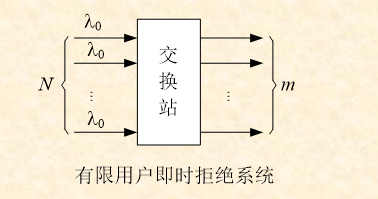
\includegraphics[width=0.7\linewidth]{figures/screenshot031}
	\caption{}
	\label{fig:screenshot031}
\end{figure}
\begin{figure}[H]
	\centering
	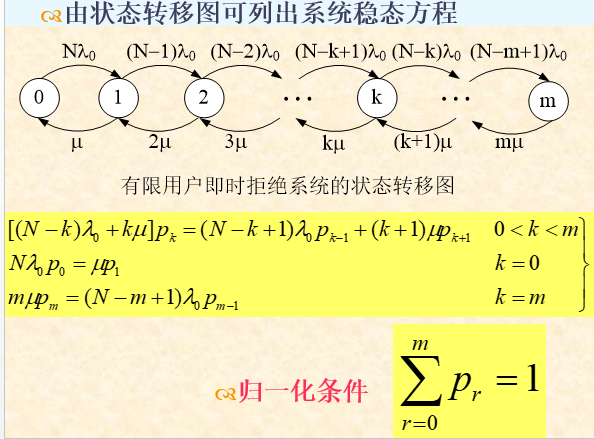
\includegraphics[width=0.7\linewidth]{figures/screenshot032}
	\caption{}
	\label{fig:screenshot032}
\end{figure}

\begin{figure}[H]
	\centering
	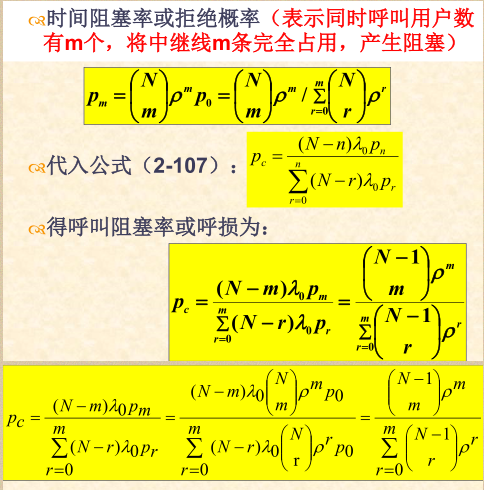
\includegraphics[width=0.5\linewidth]{figures/prove_7}
	\caption{}
	\label{fig:prove7}
\end{figure}
\subsubsection{主备线即时拒绝系统}
\begin{figure}[H]
	\centering	
		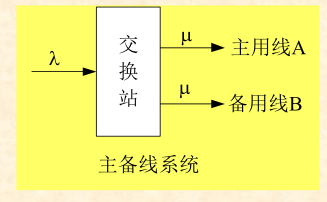
\includegraphics[width=0.4\linewidth]{figures/prove_12}
		\\	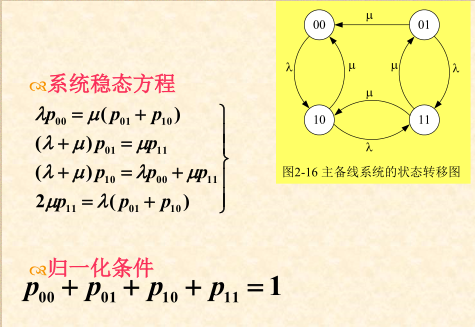
\includegraphics[width=0.5\linewidth]{figures/prove_8}
	\caption{}
	\label{fig:prove8}
\end{figure}
会求解稳态状态概率。\\
\textbf{阻塞率:}
\begin{gather}\label{key}
\text{A的阻塞率}p_{CA} = p_{10}+p_{11} \\
\text{B的阻塞率}p_{CB} = p_{01}+p_{11} \\
\text{系统阻塞}p_{c} = p_{11}
\end{gather}
\textbf{线路利用率:}
\begin{equation}\label{key}
\eta = 0\times p_0 + \frac{1}{2}p_1 + p_2 = \frac{1}{2}(p_{10}+p_{01})+p_{11}
\end{equation}
$ \frac{1}{2} $的含义为两条线路占用了一条
\subsubsection{公用备线即时拒绝系统}
\begin{figure}[H]
	\centering
	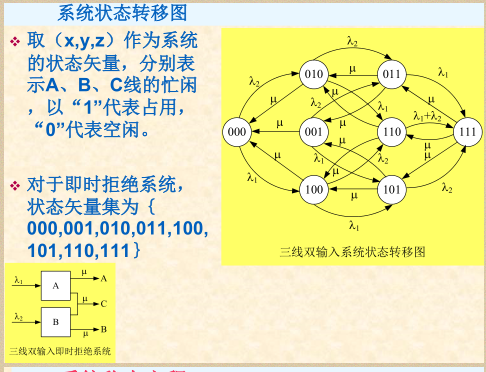
\includegraphics[width=0.5\linewidth]{figures/prove_9}
	\caption{}
	\label{fig:prove9}
\end{figure}
公用备线系统与主备线系统的比较:
公用备线系统减少一条信道,其信道利用率提高,但是呼损率有损增加。在业务量不太大的情况下,采用公用备线是很合算的。
\subsubsection{优先制排队系统}
\begin{figure}[H]
	\centering
	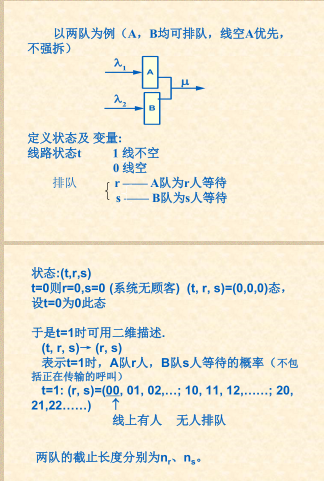
\includegraphics[width=0.5\linewidth]{figures/prove_10}
	\caption{}
	\label{fig:prove10}
\end{figure}
\begin{figure}[H]
	\centering
	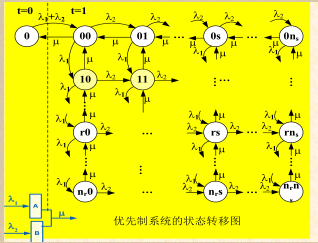
\includegraphics[width=0.5\linewidth]{figures/prove_11}
	\caption{}
	\label{fig:prove11}
\end{figure}
优先制体现在r>0时,(r,s+1)状态不能转移到(r,s)状态,因一旦线路空闲,A队将占用,就转移到(r-1,s+1)状态。按行是r变,按列是s变
\subsubsection{两次排队问题}
\begin{figure}[H]
	\centering
	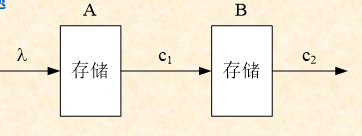
\includegraphics[width=0.7\linewidth]{figures/screenshot033}
	\caption{}
	\label{fig:screenshot033}
\end{figure}
$ \rho_1 = \frac{\lambda}{\mu} ,\rho_2 = \frac{\lambda}{\mu}$
\begin{equation}\label{key}
p_{rs} = (1-p_1)(1-p_2)p_1^rp_2^s
\end{equation}
\textbf{两个排队过程是相互独立的}\\
信息包在系统中的总时间或平均时延
\begin{equation}\label{key}
s = s_1 + s_2 = \frac{1}{\mu_1(1-p_1)} +\frac{1}{\mu_2(1-p_2)}
\end{equation}
信道的利用率分为$ p_1 $和$ p_2 $,总的利用率为:
\begin{equation}\label{key}
\eta = \frac{1}{2}(p_1+p_2)
\end{equation}
\textbf{输出定理:}
\begin{enumerate}
	\item 输出过程与输入过程相互独立,并具有同样的分布规律,即都是以$ \lambda$为均值的泊松流
	\item 使多个排队系统简化为各自独立的排队问题
	\item 如各排队系统有截止队长等限制,输出过程就无此性质
	\item 在多次排队系统中,\textbf{一旦有一个子系统不是M|M|m}问题,则这这个子系统以前的个排队过程仍可认为是相互独立的,但\textbf{在它之后就不成立了}
\end{enumerate}
\section{提高网效率的一些措施}
\subsection{大群化效应}
在\textbf{一定质量指标}的要求下,信道\textbf{统一分配会增加信道的利用率}。或者说,信道的统一分配,可比分散利用传送更多的业务量,而仍能保证一定的质量指标。这种规律就是大群化效应。
\subsubsection{示例1-M|M|m(n)即时拒绝系统}
爱尔兰公式:
\begin{figure}
	\centering
	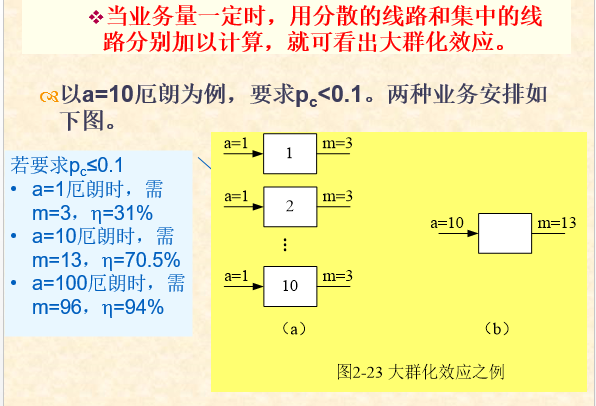
\includegraphics[width=0.7\linewidth]{figures/screenshot034}
	\caption{}
	\label{fig:screenshot034}
\end{figure}
\subsubsection{示例2-M|M|1不拒绝排队系统}
\begin{minipage}{\linewidth}

	\centering
	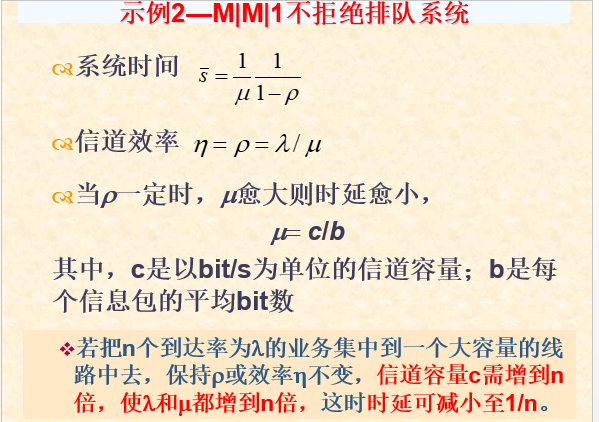
\includegraphics[width=0.5\linewidth]{figures/screenshot035}
	
	
	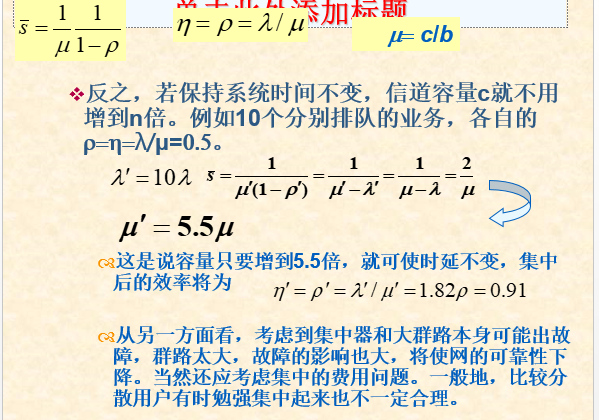
\includegraphics[width=0.5\linewidth]{figures/screenshot036}

\end{minipage}
\subsection{延迟效应}
延时、呼损和效率之间有一定的关系。延时增大,呼损明显下降,效率会显著提高。
\subsection{综合效应}
将不同性质的业务综合起来在一条线路上传输。如宽带和窄带信号的综合,数字和模拟信号的综合。可有效降低呼损率,提高信道利用率。
\begin{figure}[H]
	\centering
	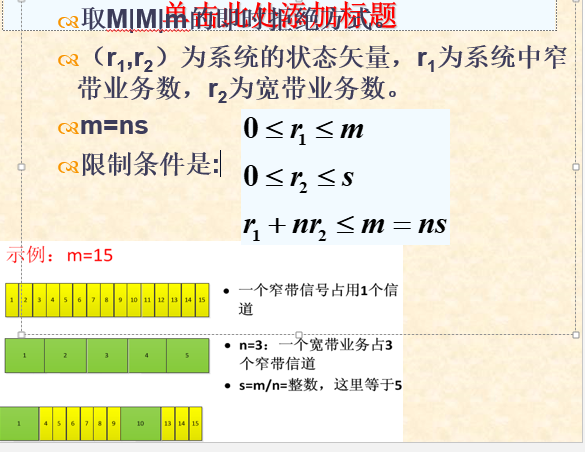
\includegraphics[width=0.7\linewidth]{figures/screenshot037}
	\caption{}
	\label{fig:screenshot037}
\end{figure}

\subsection{迂回效应}
网络中两点之间通常存在最短径与可用径的问题。最短径一般作为站间业务传输的主路由。其他径可以作为迂回路由,迂回路由除了在主路由发生故障时被采用外,还用来转接主路由中的溢出业务。\\
\textbf{利用爱尔兰公式计算呼损。}\\
\subsubsubsection{计算通过量}
\begin{figure}[H]
	\centering
	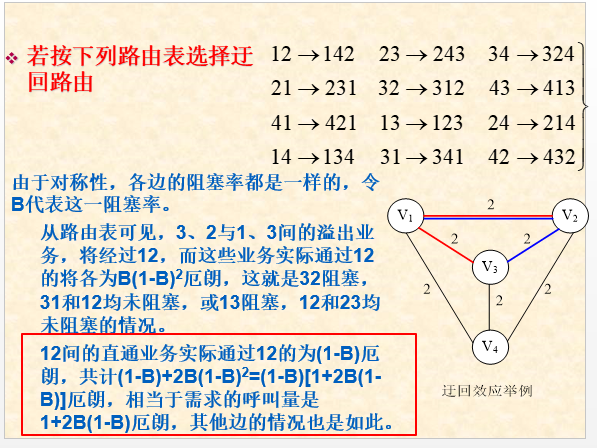
\includegraphics[width=0.7\linewidth]{figures/screenshot038}
	\caption{}
	\label{fig:screenshot038}
\end{figure}
相当于一条边除了直通的通过率$ (1-B) $还会2次被当作迂回路$ 2B(1-B)^2 $\\
使用迂回路线,可有效降低呼损率

